\documentclass[10pt,a4paper]{article}

\usepackage[top=1in, bottom=1in, left=1in, right=1in]{geometry}
\usepackage{tikz}
\usetikzlibrary{arrows.meta, calc}
\usepackage{amsmath}
\usepackage{booktabs}
\usepackage{xcolor}
\usepackage{caption}
\usepackage{subcaption}
\usepackage{float}
\usepackage{enumitem}
\usepackage{titlesec}
\usepackage[hidelinks]{hyperref}

\linespread{1.05}

\captionsetup{font=small, skip=6pt}
\setlength{\parskip}{5pt}
\setlength{\parindent}{0pt}
\setlength{\floatsep}{12pt}
\setlength{\textfloatsep}{14pt}
\setlength{\abovecaptionskip}{6pt}
\setlength{\belowcaptionskip}{2pt}
\setlength{\intextsep}{12pt}

\renewcommand{\arraystretch}{1.25}

\titleformat{\section}{\bfseries\normalsize}{}{0em}{}[\vspace{-0.2em}\rule{\linewidth}{0.5pt}]
\titleformat{\subsection}{\bfseries\small}{}{0em}{}
\titlespacing{\section}{0pt}{14pt}{5pt}
\titlespacing{\subsection}{0pt}{8pt}{3pt}

% -----------------------------------------------------------------------
\begin{document}

\begin{center}
  {\Large\textbf{UnderwaterLink}}\\[0.3em]
  {\normalsize\textbf{Reliable Smartphone-to-Smartphone Optical Communication Underwater}}\\[0.5em]
  {\small
    Vishrut Ramraj (2023A7PS0352G)\quad
    Ragav Krishna Ramesh (2023A7PS0415G)\quad
    Divyam Gupta (2023A7PS0423G)\\[0.2em]
    \textit{Problem Statement: Reliable Underwater Communication Using Smartphones}\quad
    $\cdot$\quad\textit{Proposed by Prof.\ Arnab Paul}
  }
\end{center}
\vspace{0.5em}\hrule\vspace{0.7em}

\noindent\textbf{Abstract.}\;
We propose \emph{UnderwaterLink}, a native Android application enabling reliable data
transfer between two smartphones underwater using only the built-in flashlight (transmitter)
and camera (receiver). Our system addresses the four main failure modes of underwater
optical communication---absolute-brightness fluctuation, device motion, ambient-light
interference, and inter-symbol interference---through a co-designed, layered stack:
\textbf{4-ary Pulse Width Modulation} (PWM) at the physical layer,
\textbf{Huffman source coding} approaching the Shannon entropy bound,
a \textbf{temporal-saliency adaptive Region-of-Interest (ROI) tracker} at the receiver,
and a \textbf{Stop-and-Wait ARQ} link layer with CRC8 error detection.
Critically, the design embraces water scattering as a detection aid, not an obstacle.

\vspace{0.5em}
% -----------------------------------------------------------------------
\section{1.\enspace Introduction \& Motivation}

The U-Flash paper (IMWUT 2024)~\cite{uflash} demonstrated that commercial smartphones can
communicate underwater using only the flashlight and rolling-shutter camera, and that light
scattering---typically viewed as harmful---actually \emph{enlarges} the camera's effective
Region of Interest, improving detectability. Despite this, raw reliability remains poor due to:
(i)~rapid brightness fluctuations from turbidity and ambient light;
(ii)~motion between devices causing loss of lock;
(iii)~inter-symbol interference from light-scattering blur; and
(iv)~the absence of a shared clock between sender and receiver.
\textbf{UnderwaterLink} addresses each failure mode with a dedicated mechanism at the
appropriate protocol layer, rather than applying a single post-hoc fix.

% -----------------------------------------------------------------------
\section{2.\enspace System Architecture}

\begin{figure}[h]
\centering
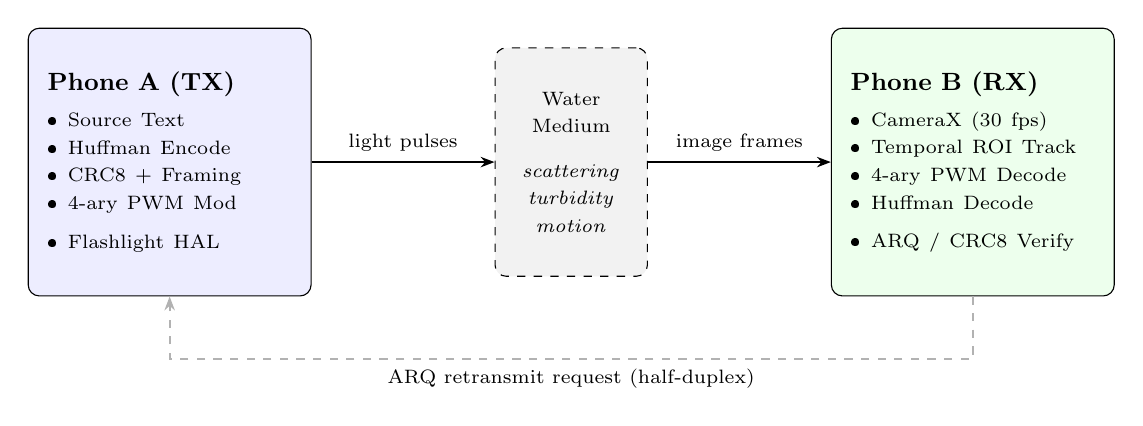
\begin{tikzpicture}[arr/.style={-{Stealth[length=5pt]}, thick, font=\scriptsize}]

  % ----- TX box -----
  \node[draw, rounded corners=4pt, fill=blue!7, text width=3.1cm,
        minimum height=3.4cm, align=left, inner sep=7pt] at (0,0) (tx) {
    \small\textbf{Phone A (TX)}\\[5pt]
    \scriptsize
    \textbullet~Source Text\\[2pt]
    \textbullet~Huffman Encode\\[2pt]
    \textbullet~CRC8 + Framing\\[2pt]
    \textbullet~4-ary PWM Mod\\[2pt]
    \textbullet~Flashlight HAL
  };

  % ----- Water block -----
  \node[draw, dashed, rounded corners=4pt, fill=gray!10, text width=1.7cm,
        minimum height=2.9cm, align=center, font=\scriptsize] at (5.1,0) (water) {
    Water\\[2pt]Medium\\[8pt]
    \textit{scattering}\\[2pt]
    \textit{turbidity}\\[2pt]
    \textit{motion}
  };

  % ----- RX box -----
  \node[draw, rounded corners=4pt, fill=green!7, text width=3.1cm,
        minimum height=3.4cm, align=left, inner sep=7pt] at (10.2,0) (rx) {
    \small\textbf{Phone B (RX)}\\[5pt]
    \scriptsize
    \textbullet~CameraX (30 fps)\\[2pt]
    \textbullet~Temporal ROI Track\\[2pt]
    \textbullet~4-ary PWM Decode\\[2pt]
    \textbullet~Huffman Decode\\[2pt]
    \textbullet~ARQ / CRC8 Verify
  };

  % ----- Forward arrows -----
  \draw[arr] (tx.east) -- node[above, font=\scriptsize] {light pulses} (water.west);
  \draw[arr] (water.east) -- node[above, font=\scriptsize] {image frames} (rx.west);

  % ----- ARQ feedback arrow (below boxes) -----
  \coordinate (low) at (0,-2.5);
  \draw[arr, dashed, gray!60]
    (rx.south) -- (rx.south |- low) --
    node[below, font=\scriptsize, black, midway] {ARQ retransmit request (half-duplex)}
    (tx.south |- low) -- (tx.south);

\end{tikzpicture}
\caption{UnderwaterLink full-stack architecture.
         Roles are symmetric; each phone may switch between TX and RX via half-duplex token passing.}
\label{fig:arch}
\end{figure}

% -----------------------------------------------------------------------
\section{3.\enspace Physical Layer: 4-ary Pulse Width Modulation}

\subsection{Design Rationale}
Simple On-Off Keying (OOK) fails underwater because decoding requires an \emph{absolute}
brightness threshold that fluctuates with turbidity, distance, and ambient light.
Pulse Width Modulation encodes information in the \emph{duration} of each ON pulse relative
to a fixed 100\,ms symbol period---the receiver only asks ``was the pulse long or short?'',
making it inherently immune to absolute brightness changes.

Using four distinct ON durations (4-ary PWM) rather than two doubles the effective bit rate
to 20\,bps without shrinking any pulse below the torch hardware consistency floor
($\approx$20\,ms). All four levels were validated on a real device; measured inter-level
separation margins are 8.4\,ms / 14.5\,ms / 14.9\,ms---all clearly positive.

\begin{figure}[h]
\centering
\begin{subfigure}[t]{0.38\linewidth}
\centering
\small
\begin{tabular}{ccccc}
\toprule
\textbf{Sym} & \textbf{Bits} & \textbf{ON} & \textbf{OFF} & \textbf{Meas.\ $\sigma$} \\
\midrule
$S_0$ & 00 & 25\,ms & 75\,ms & 1.38\,ms \\
$S_1$ & 01 & 40\,ms & 60\,ms & 0.04\,ms \\
$S_2$ & 10 & 55\,ms & 45\,ms & $<$0.01\,ms \\
$S_3$ & 11 & 70\,ms & 30\,ms & $<$0.01\,ms \\
\bottomrule
\end{tabular}
\subcaption{Symbol table. Period fixed at 100\,ms.
Measured $\sigma$ from a 198-char real-device test.}
\label{tab:pwm}
\end{subfigure}
\hfill
\begin{subfigure}[t]{0.58\linewidth}
\centering
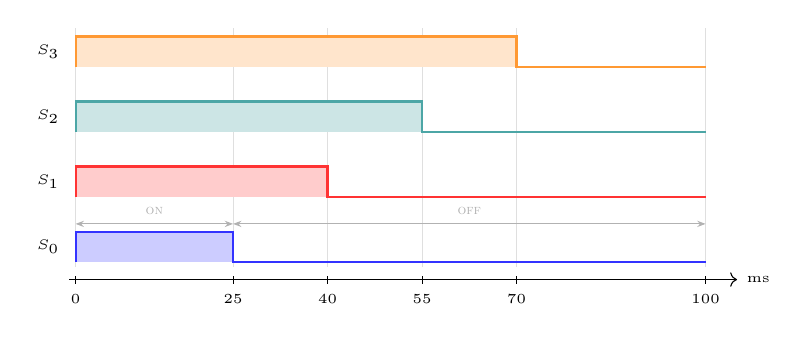
\begin{tikzpicture}[xscale=0.80, yscale=0.70]
  \def\H{0.55}   % pulse height
  \def\rs{1.18}  % row spacing

  % Dashed vertical reference lines
  \foreach \x in {0, 2.5, 4.0, 5.5, 7.0, 10.0}
    \draw[gray!25, thin] (\x, -0.1) -- (\x, {3*\rs+\H+0.15});

  % S0: ON=25ms
  \fill[blue!20] (0,0) rectangle (2.5,\H);
  \draw[blue!80, thick] (0,0)--(0,\H)--(2.5,\H)--(2.5,0)--(10,0);
  \node[left, font=\tiny] at (-0.1,{\H/2}) {$S_0$};

  % S1: ON=40ms
  \fill[red!20] (0,\rs) rectangle (4.0,{\rs+\H});
  \draw[red!80, thick] (0,\rs)--(0,{\rs+\H})--(4.0,{\rs+\H})--(4.0,\rs)--(10,\rs);
  \node[left, font=\tiny] at (-0.1,{\rs+\H/2}) {$S_1$};

  % S2: ON=55ms
  \fill[teal!20] (0,{2*\rs}) rectangle (5.5,{2*\rs+\H});
  \draw[teal!70, thick] (0,{2*\rs})--(0,{2*\rs+\H})--(5.5,{2*\rs+\H})--(5.5,{2*\rs})--(10,{2*\rs});
  \node[left, font=\tiny] at (-0.1,{2*\rs+\H/2}) {$S_2$};

  % S3: ON=70ms
  \fill[orange!20] (0,{3*\rs}) rectangle (7.0,{3*\rs+\H});
  \draw[orange!80, thick] (0,{3*\rs})--(0,{3*\rs+\H})--(7.0,{3*\rs+\H})--(7.0,{3*\rs})--(10,{3*\rs});
  \node[left, font=\tiny] at (-0.1,{3*\rs+\H/2}) {$S_3$};

  % Time axis
  \draw[->] (-0.1,-0.32) -- (10.5,-0.32) node[right, font=\tiny] {ms};
  \foreach \x/\lbl in {0/0, 2.5/25, 4.0/40, 5.5/55, 7.0/70, 10.0/100} {
    \draw (\x,-0.26)--(\x,-0.40);
    \node[below, font=\tiny] at (\x,-0.42) {\lbl};
  }

  % ON / OFF labels for S0
  \draw[{Stealth[length=3pt]}-{Stealth[length=3pt]}, gray!60, thin]
    (0,{\H+0.14}) -- node[above,font=\tiny] {\textsc{on}} (2.5,{\H+0.14});
  \draw[{Stealth[length=3pt]}-{Stealth[length=3pt]}, gray!60, thin]
    (2.5,{\H+0.14}) -- node[above,font=\tiny] {\textsc{off}} (10,{\H+0.14});

\end{tikzpicture}
\subcaption{PWM waveforms (one 100\,ms period). Shaded region = ON duration.}
\label{fig:waveform}
\end{subfigure}
\caption{4-ary PWM encoding: information is carried in ON duration, not brightness.}
\label{fig:pwm}
\end{figure}

\subsection{Transmitter Reliability}
TX runs on a dedicated thread at \texttt{THREAD\_PRIORITY\_URGENT\_AUDIO}.
Each symbol's firing time is computed as an absolute offset from the transmission start
using \texttt{SystemClock.elapsedRealtimeNanos()}, and the thread busy-waits until that
nanosecond---preventing jitter accumulation across symbols.
Every frame is preceded by a two-toggle \emph{warmup} (to initialise the torch HAL),
followed by a \textbf{200\,ms ON start marker} (uniquely longer than any data symbol)
then 100\,ms OFF for receiver clock synchronisation.

% -----------------------------------------------------------------------
\section{4.\enspace Source Coding: Approaching the Shannon Limit}

Raw ASCII assigns every character 8 bits regardless of its frequency in natural language.
For English text, the Shannon entropy is $H \approx 4.5$\,bits/char---nearly half of 8\,bits/char.
We bridge this gap with \textbf{Huffman coding}: a codebook derived from English character
frequency statistics assigns short codewords (e.g.\ \texttt{e} $\to$ 2--3 bits) to frequent
characters and longer codewords to rare ones.
Huffman codes are provably optimal for symbol-by-symbol lossless compression, reducing
transmitted symbol count by $\sim$44\% compared to raw ASCII.

An alternative we are exploring is a \textbf{Morse-inspired variable-length encoding}:
the 12 most frequent English letters map to 1--2 symbols; the rest to 3--4.
This has a compact, fixed codebook with zero per-message overhead, at a slight efficiency
cost relative to Huffman, but is resilient to codebook synchronisation errors.

\textbf{Practical impact:} Fewer transmitted symbols mean shorter transmission time,
fewer channel error opportunities, and lower ARQ overhead---all critical in a high-BER
underwater channel.

% -----------------------------------------------------------------------
\section{5.\enspace Camera Receiver: Temporal Saliency \& Adaptive ROI}

Standard brightness-based tracking (brightest pixel, blob detection) fails underwater
because sunlight reflections and turbidity create bright, moving regions visually
indistinguishable from the signal.
Our receiver does not track \emph{brightness}---it tracks \textbf{temporal modulation}:
regions that are \emph{periodically changing} are the signal; static bright patches are noise.

\subsection*{Four-Phase Algorithm}
\begin{enumerate}[leftmargin=*, itemsep=4pt, topsep=5pt, label=\textbf{Phase \arabic*.}]

\item \textbf{Global Activity Map.}
Each CameraX frame's luminance plane is downsampled to a coarse grid
(e.g.\ 64$\times$48 blocks). Per block, a rolling history of min/max brightness
over 0.5\,s yields \texttt{DynamicRange = Max $-$ Min}.
Blocks exceeding a noise threshold are marked ``active.''
Static sunlight has consistently high brightness but near-zero dynamic range once
time-averaged; a blinking flashlight has large dynamic range.
Connected-components analysis groups adjacent active blocks into candidate clusters,
discarding those smaller than a minimum size to eliminate sensor noise.

\item \textbf{Pattern Validation.}
For each candidate cluster, the time-domain brightness sequence is compared against
the known calibration signature (\texttt{C1}: 200\,ms ON / 100\,ms OFF, repeating).
Clusters failing this timing check---waving hands, wave turbulence---are discarded.
Lock is declared after two matching cycles.

\item \textbf{ROI Lock.}
The validated cluster's bounding box (plus 20\% padding) becomes the ROI.
The receiver records \texttt{RefBrightness} (mean ON-state luminance) and
\texttt{RefDarkness} (mean OFF-state luminance) as adaptive decoding thresholds.

\item \textbf{Sample-and-Hold Tracking.}
During data reception, the ROI position is updated via a low-pass filter on
the light centroid \emph{only when the signal is ON}:
\[
  \mathrm{ROI} \;\leftarrow\; 0.8\cdot\mathrm{ROI} \;+\; 0.2\cdot\mathrm{Centroid}_{\mathrm{ON}}
\]
When the signal is OFF (30--75\,ms per symbol), the ROI is \textbf{frozen}---no
position update is made.
Tracking the centroid of a dark frame means tracking noise; freezing prevents
the ROI from drifting away during the frequent OFF gaps of 4-ary PWM.
\end{enumerate}

\noindent\textbf{Exploiting scattering:}
Water scattering blurs the flashlight into an extended halo.
Our coarse-grid activity map aggregates this enlarged energy naturally,
and centroid-based tracking finds the halo's centre---yielding \emph{more} stable
ROI lock than tracking a sharp point source would.
We therefore treat scattering as a feature, consistent with the U-Flash insight.

% -----------------------------------------------------------------------
\section{6.\enspace Link Layer: Calibration \& Reliable Delivery}

\begin{figure}[h]
\centering
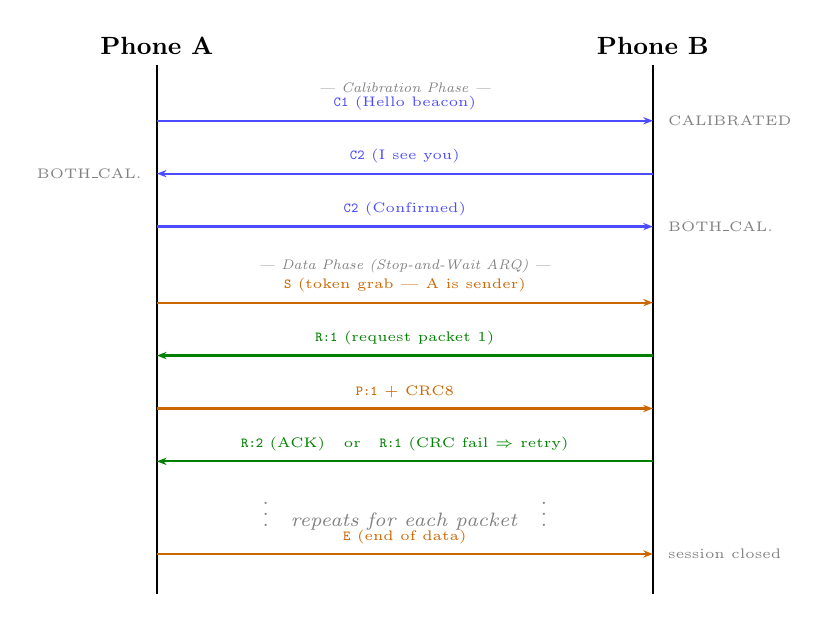
\begin{tikzpicture}[xscale=1.05, yscale=0.84, font=\scriptsize,
  arr/.style={-{Stealth[length=3.5pt]}, thick}]

  % Lifelines
  \draw[thick] (0,0) node[above, font=\small\bfseries]{Phone A} -- (0,-8.0);
  \draw[thick] (6,0) node[above, font=\small\bfseries]{Phone B} -- (6,-8.0);

  % ---- Calibration ----
  \node[gray, font=\tiny\itshape] at (3,-0.35) {--- Calibration Phase ---};

  \draw[arr, blue!70] (0,-0.85) -- (6,-0.85)
    node[midway, above, font=\tiny] {\texttt{C1} (Hello beacon)};
  \node[gray, font=\tiny, right=2pt] at (6,-0.85) {CALIBRATED};

  \draw[arr, blue!70] (6,-1.65) -- (0,-1.65)
    node[midway, above, font=\tiny] {\texttt{C2} (I see you)};
  \node[gray, font=\tiny, left=2pt] at (0,-1.65) {BOTH\_CAL.};

  \draw[arr, blue!70] (0,-2.45) -- (6,-2.45)
    node[midway, above, font=\tiny] {\texttt{C2} (Confirmed)};
  \node[gray, font=\tiny, right=2pt] at (6,-2.45) {BOTH\_CAL.};

  % ---- Data Phase ----
  \node[gray, font=\tiny\itshape] at (3,-3.05) {--- Data Phase (Stop-and-Wait ARQ) ---};

  \draw[arr, orange!80!black] (0,-3.6) -- (6,-3.6)
    node[midway, above, font=\tiny] {\texttt{S} (token grab --- A is sender)};

  \draw[arr, green!50!black] (6,-4.4) -- (0,-4.4)
    node[midway, above, font=\tiny] {\texttt{R:1} (request packet 1)};

  \draw[arr, orange!80!black] (0,-5.2) -- (6,-5.2)
    node[midway, above, font=\tiny] {\texttt{P:1} + CRC8};

  \draw[arr, green!50!black] (6,-6.0) -- (0,-6.0)
    node[midway, above, font=\tiny] {\texttt{R:2} (ACK)\quad or\quad\texttt{R:1} (CRC fail $\Rightarrow$ retry)};

  \node[font=\scriptsize, gray] at (3,-6.7) {$\vdots$\quad\emph{repeats for each packet}\quad$\vdots$};

  \draw[arr, orange!80!black] (0,-7.4) -- (6,-7.4)
    node[midway, above, font=\tiny] {\texttt{E} (end of data)};
  \node[gray, font=\tiny, right=2pt] at (6,-7.4) {session closed};

\end{tikzpicture}
\caption{Communication sequence diagram.
The randomised backoff (not shown) resolves the initial discovery problem.
The 3-way handshake establishes bidirectional optical lock.
The ARQ loop repeats until \texttt{E} is received.}
\label{fig:seq}
\end{figure}

\textbf{Calibration (Discovery).}
Both phones start in an \texttt{UNCALIBRATED} state and independently choose---with random
probability---either to transmit \texttt{C1} then listen, or to listen only.
This randomised backoff breaks transmission symmetry, ensuring one phone eventually
hears the other's \texttt{C1} even if they begin simultaneously.
A successful 3-way handshake advances both to \texttt{BOTH\_CALIBRATED}, and both sides
learn each other's signal characteristics (\texttt{RefBrightness}, timing).
Calibration failure (timeout) reverts both phones to \texttt{UNCALIBRATED} for retry
up to \texttt{MAX\_RETRIES}.

\textbf{Stop-and-Wait ARQ.}
The token holder (sender) transmits one packet at a time: a Huffman-encoded payload
plus a CRC8 checksum.
The receiver sends \texttt{R:n+1} on success, or \texttt{R:n} on CRC8 failure to request
retransmission of the same packet.
This guarantees zero packet loss at the cost of round-trip latency, acceptable for a
high-BER underwater channel.
Packet sizes are chosen so that ARQ overhead remains below 30\% of total
transmission time.

% -----------------------------------------------------------------------
\section{7.\enspace Reliability Engineering: Failure Modes \& Mitigations}

\begin{center}\small\setlength{\tabcolsep}{8pt}
\begin{tabular}{lll}
\toprule
\textbf{Failure Mode} & \textbf{Mitigation} & \textbf{Layer} \\
\midrule
Absolute brightness fluctuation & PWM: duration-based, not amplitude-based & PHY \\
Torch HAL timing jitter & Absolute wall-clock scheduling; \texttt{URGENT\_AUDIO} thread & PHY \\
Static ambient light / reflections & Temporal activity map: modulation $\neq$ brightness & RX \\
Signal absent during OFF gaps & Sample-and-Hold ROI freeze & RX \\
Diver motion between devices & Centroid-based low-pass ROI update (ON frames only) & RX \\
Packet corruption (bit errors) & CRC8 per packet + automatic ARQ retransmit & Link \\
Transmission efficiency & Huffman coding ($\sim$44\% symbol count reduction) & Source \\
Discovery collision & Randomised backoff + 3-way handshake & Link \\
\bottomrule
\end{tabular}
\end{center}

% -----------------------------------------------------------------------
\section{8.\enspace Evaluation Plan}

We target the quantitative metrics specified in the problem statement:

\begin{itemize}[leftmargin=*, topsep=5pt, itemsep=4pt]
  \item \textbf{Bit Error Rate (BER):} measured before and after ARQ correction,
        under still-water and $\pm$10\,cm lateral motion, at distances of
        0.5\,m, 1.0\,m, and 1.5\,m in a water tank.

  \item \textbf{Frame decode success rate:} fraction of messages received
        intact across 50 repeated trials per condition.

  \item \textbf{Effective throughput:} user-data bits per second, accounting
        for Huffman compression, ARQ overhead, and framing overhead.

  \item \textbf{Ablation comparison:}
        Raw OOK $\to$ 4-ary PWM $\to$ 4-ary PWM + Huffman, isolating each
        design decision's contribution to BER reduction.

  \item \textbf{ROI tracker robustness:} lock-acquisition time and lock-loss
        rate as a function of ambient light intensity and diver motion speed.
\end{itemize}

% -----------------------------------------------------------------------
\section{9.\enspace Conclusion}

UnderwaterLink attacks underwater optical communication reliability through a
co-designed, layered architecture.
At the physical layer, 4-ary PWM provides amplitude-invariant modulation with
validated sub-millisecond timing accuracy.
At the source layer, Huffman coding closes the gap to the Shannon entropy bound,
reducing channel exposure by $\sim$44\%.
At the receiver, temporal-saliency ROI tracking and Sample-and-Hold freezing exploit
water scattering rather than fighting it.
At the link layer, Stop-and-Wait ARQ with CRC8 guarantees end-to-end delivery.
Every design decision directly targets a documented failure mode of the underwater
smartphone channel, with no external hardware required beyond the stock flashlight and camera.

\begin{thebibliography}{9}
\bibitem{uflash}
  Y.\ Ding \emph{et al.},
  ``U-Flash: Improving Underwater Optical Communication by Scattering Effect,''
  in \emph{Proc.\ ACM Interact.\ Mob.\ Wearable Ubiquitous Technol.\ (IMWUT)}, 2024.
\end{thebibliography}

\end{document}
